% !TEX root=ricardo_draft.tex
% In this section we evaluate our framework for modeling fairness.

%%%% TODO!!! ADD COMMENT THAT WE NEED Y TO LEARN THE CAUSAL MODEL!!!!!

\section*{S1 Population Level vs Individual Level Causal Effects}
\label{sec:individual}

As discussed in Section~\ref{sec:count_fair}, counterfactual fairness
is an individual-level definition. This is fundamentally different
from comparing different units that happen to share the same
“treatment” $A = a$ and coincide on the values of $X$. To see in
detail what this means, consider the following thought experiment.

Let us assess the causal effect of $A$ on $\hat Y$ by controlling
$A$ at two levels, $a$ and $a'$. In Pearl's notation, where ``$do(A = a)$''
expresses an intervention on $A$ at level $a$, we have that
\begin{equation}
\label{eq:ace}
\mathbb{E}[\hat Y\ |\ do(A = a), X = x] - \mathbb{E}[\hat Y\ |\ do(A = a'), X = x],
\end{equation}
is a measure of causal effect, sometimes called the average causal
effect (ACE). It expresses the change that is expected when we
intervene on $A$ while observing the attribute set $X = x$, under two
levels of treatment. If this effect is non-zero, $A$ is considered to
be a cause of $\hat Y$.

This raises a subtlety that needs to be addressed: in general, this
effect will be non-zero {\it even if $\hat Y$ is counterfactually
  fair}. This may sound counter-intuitive: protected attributes such
as race and gender are causes of our counterfactually fair decisions.

In fact, this is not a contradiction, as the ACE in Equation
(\ref{eq:ace}) is different from counterfactual effects. The ACE
contrasts two independent exchangeable units of the population, and it
is a perfectly valid way of performing decision analysis. However, the
value of $X = x$ is affected by different background variables
corresponding to different individuals. That is, the causal effect
(\ref{eq:ace}) contrasts two units that receive different treatments
but which happen to coincide on $X = x$. To give a synthetic example,
imagine the simple structural equation
\[
X = A + U.
\]

The ACE quantifies what happens among people with $U = x -
a$ against people with $U' = x - a'$. If, for instance, $\hat Y =
\lambda U$ for $\lambda \neq 0$, then the effect \eqref{eq:ace}
is $\lambda(a - a') \neq 0$.

Contrary to that, the counterfactual difference is zero.
That is,
\[
\mathbb{E}[\hat Y_{A \leftarrow a}(U)\ |\ A = a, X = x] -
\mathbb{E}[\hat Y_{A \leftarrow a'}(U)\ |\ A = a, X = x] =
\lambda U - \lambda U = 0.
\]

In another perspective, we can interpret the above just as if we had
{\it measured} $U$ from the beginning rather than performing
abduction. We then generate $\hat Y$ from some $g(U)$, so $U$ is the
within-unit cause of $\hat Y$ and not $A$.

If $U$ cannot be deterministically derived from $\{A = a, X = x\}$,
the reasoning is similar. By abduction, the distribution of $U$ will
typically depend on $A$, and hence so will $\hat Y$ when marginalizing
over $U$. Again, this seems to disagree with the intuition that our
predictor should be not be caused by $A$. However, this once again is
a comparison {\it across individuals}, not within an individual. 

It is this balance among $(A, X, U)$ that explains, in the examples
of Section~\ref{sec:further_examples}, why some predictors are
counterfactually fair even though they are functions of the same
variables $\{A, X\}$ used by unfair predictors: such functions must
correspond to particular ways of balancing the observables that, by
way of the causal assumptions, cancel out the effect of $A$.

\noindent {\bf More on conditioning and alternative definitions.} As discussed in
Example 4.4.4 of \citet{pearl:16}, a different proposal for
assessing fairness can be defined via the following concept:
\begin{define}[Probability of sufficiency]
  We define the probability of event $\{ A = a \}$ being a
  \emph{sufficient cause} for our
  decision $\hat Y$, contrasted against $\{ A = a' \}$, as
\begin{align}
  P(\hat Y_{A \leftarrow a'\ }(U) \neq y\ |\ X = x, A = a, \hat Y = y).
  \label{eq:sufficiency}
\end{align}
\end{define}

We can then, for instance, claim that $\hat Y$ is a fair predictor if
this probability is below some pre-specified bound for all $(x, a,
a')$. The shortcomings of this definition come from its original
motivation: to {\it explain} the behavior of an {\it existing}
decision protocol, where $\hat Y$ is the current practice and which in a
unclear way is conflated with $Y$. The implication is that if $\hat Y$
is to be designed instead of being a natural measure of existing
behaviour, then we are using $\hat Y$ itself as evidence for the
background variables $U$. This does not make sense if $\hat Y$ is
yet to be designed by us. If $\hat Y$ is to be interpreted as $Y$, then this
does not provide a clear recipe on how to build $\hat Y$: while we can
use $Y$ to learn a causal model, we cannot use it to collect training
data evidence for $U$ {\it as the outcome $Y$ will not be available to
  us at prediction time}. For this reason, we claim that while
probability of sufficiency is useful as a way of assessing an existing
decision making process, it is not as natural as counterfactual
fairness in the context of machine learning.

\noindent {\bf Approximate fairness and model validation.} The notion
of probability of sufficiency raises the question on how to define
approximate, or high probability, counterfactual fairness. This is an
important question that we address in \citep{russell:17}. Before
defining an approximation, it is important to first expose in detail
what the exact definition is, which is the goal of this paper.

We also do not address the validation of the causal assumptions used
by the input causal model of the {\sc FairLearning} algorithm in
Section \ref{sec:algorithm}. The reason is straightforward: this
validation is an entirely self-contained step of the implementation of
counterfactual fairness. An extensive literature already exists in
this topic which the practitioner can refer to (a classic account for
instance is \cite{bollen:93}), and which can be used as-is in our
context.

The experiments performed in Section \ref{sec:experiments} can be
criticized by the fact that they rely on a model that obeys our
assumptions, and ``obviously'' our approach should work better than
alternatives. This criticism is not warranted: in machine learning,
causal inference is typically assessed through simulations which
assume that the true model lies in the family covered by the
algorithm.  Algorithms, including {\sc FairLearning}, are justified in
the population sense. How different competitors behave with finite
sample sizes is the primary question to be studied in an empirical
study of a new concept, where we control for the correctness of the
assumptions. Although sensitivity analysis is important, there are
many degrees of freedom on how this can be done. Robustness issues are
better addressed by extensions focusing on approximate versions of 
counterfactual fairness. This will be covered in later work.

\noindent {\bf Stricter version.} For completeness of exposition,
notice that the definition of counterfactual fairness could be
strengthened to
\begin{align}
  \label{eq:stricter}
  P(\{\hat Y_{A \leftarrow a}(U) = \hat Y_{A \leftarrow a'}(U)\} = 1\ |\ X = x, A = a).
\end{align}

\noindent This is different from the original definition in the case
where $\hat Y(U)$ is a random variable with a different source of
randomness for different counterfactuals (for instance, if $\hat Y$ is
given by some black-box function of $U$ with added noise that is
independent across each countefactual value of $A$). In such a
situation, the event $\{\hat Y_{A \leftarrow a}(U) = \hat Y_{A
  \leftarrow a'}(U)\}$ will itself have probability zero even if
$P(\hat Y_{A \leftarrow a}(U) = y\ |\ X = x, A = a) = P(\hat Y_{A
  \leftarrow a'}(U) = y\ |\ X = x, A = a)$ for all $y$. We do not
consider version (\ref{eq:stricter}) as in our view it does not feel
as elegant as the original, and it is also unclear whether adding an
independent source of randomness fed to $\hat Y$ would itself be
considered unfair. Moreover, if $\hat Y(U)$ is assumed to be a
deterministic function of $U$ and $X$, as in {\sc FairLearning}, then
the two definitions are the same\footnote{Notice that $\hat Y(U)$ is
  itself a random variable if $U$ is, but the source of randomness,
  $U$, is the same across all counterfactuals.}. Informally, this
stricter definition corresponds to a notion of ``almost surely
equality'' as opposed to ``equality in distribution.'' Without
assuming that $\hat Y$ is a deterministic function of $U$ and $X$,
even the stricter version does not protect us against measure zero events
where the counterfactuals are different. The definition of
counterfactual fairness concisely emphasizes that $U$ can be a random
variable, and clarifies which conditional distribution it follows. Hence, it is our
preferred way of introducing the concept even though it does not
explicit suggests whether $\hat Y(U)$ has random inputs besides $U$.

\section*{S2 Relation to Demographic Parity}
%
Consider the graph $A \rightarrow X \rightarrow Y$. In general, if
$\hat Y$ is a function of $X$ only, then $\hat Y$ need not obey
demographic parity, i.e.
\begin{align}
  P(\hat Y\ |\ A = a) \neq P(\hat Y\ |\ A = a'),\nonumber
\end{align}
\noindent where, since $\hat Y$ is a function of $X$, the
probabilities are obtained by marginalizing over $P(X\ |\ A = a)$ and
$P(X\ |\ A = a')$, respectively.

If we postulate a structural equation $X = \alpha A + e_X$, then given
$A$ and $X$ we can deduce $e_X$. If $\hat Y$ is a function of $e_X$
only and, by assumption, $e_X$ is marginally independent of $A$, then
$\hat Y$ is marginally independent of $A$: this follows the
interpretation given in the previous section, where we interpret $e_X$
as ``known'' despite being mathematically deduced from the
observation $(A = a, X = x)$. Therefore, the assumptions imply that
$\hat Y$ will satisfy demographic parity, and that can be falsified.
By way of contrast, if $e_X$ is not uniquely identifiable from the
structural equation and $(A, X)$, then the distribution of $\hat Y$
depends on the value of $A$ as we marginalize $e_X$, and demographic
parity will not follow. This leads to the following:
%
\begin{lem}
If all background variables $U' \subseteq U$ in the definition of
$\hat Y$ are determined from $A$ and $X$,
and all observable variables in the definition of $\hat Y$ are
independent of $A$ given $U'$, then $\hat Y$ satisfies demographic
parity.
% If the conditions fail, then $\hat Y$ will not satisfy demographic parity in general. 
\end{lem}
Thus, counterfactual fairness can be thought of as a counterfactual
analog of demographic parity, as present in the Red Car example further discussed
in the next section.

\section*{S3 Examples Revisited}

In Section \ref{sec:further_examples}, we discussed two examples. We
reintroduce them here briefly, add a third example, and explain some
consequences of their causal structure to the design of
counterfactually fair predictors.

\paragraph{Scenario 1: The Red Car Revisited.}
In that scenario, the structure $A \rightarrow X \leftarrow U
\rightarrow Y$ implies that $\hat Y$ should not use either $X$ or
$A$. On the other hand, it is acceptable to use $U$.  It is
interesting to realize, however, that since $U$ is related to $A$ and
$X$, there will be some association between $Y$ and $\{A, X\}$ as
discussed in Section S1. In particular, if the structural equation for
$X$ is linear, then $U$ is a linear function of $A$ and $X$, and as
such $\hat Y$ will also be a function of both $A$ and $X$. This is not
a problem, as it is still the case that the model implies that this is
merely a functional dependence that disappears by conditioning on a
postulated latent attribute $U$. Surprisingly, we must make $\hat Y$ a
indirect function of $A$ if we want a counterfactually fair predictor,
as shown in the following Lemma.

  %
\begin{lem}
Consider a linear model with the structure in
Figure~\ref{figure.simple_models}(a).  Fitting a linear predictor to
$X$ \emph{only} is not counterfactually fair, while the same algorithm
will produce a fair predictor using \emph{both} $A$ and $X$.
\end{lem}

\begin{proof}
As in the definition, we will consider the population case, where the
joint distribution is known. Consider the case where the equations
described by the model in Figure~\ref{figure.simple_models}(a)
are deterministic and linear:
\begin{align}
X = \alpha A + \beta U, \;\;\;\; Y = \gamma U. \nonumber
\end{align}
Denote the variance of $U$ as $v_U$, the variance of $A$ as $v_A$, and
assume all coefficients are non-zero. The predictor $\hat Y(X)$
defined by least-squares regression of $Y$ on \emph{only} $X$ is given
by $\hat Y(X) \equiv \lambda X$, where $\lambda = Cov(X, Y) / Var(X)
\!=\! \beta\gamma v_U / (\alpha^2 v_A + \beta^2 v_U) \neq 0$. This 
predictor follows the concept of fairness through unawareness.

We can test whether a predictor $\hat{Y}$ is counterfactually fair
by using the procedure described in Section~\ref{subsec:cmc}:

%\begin{itemize}
{\em (i)} Compute $U$ given observations of $X,Y,A$; %, by solving for $U$.
{\em (ii)} Substitute the equations involving $A$ with an interventional value $a'$; 
% (i.e., this says: `what happens if the race of an individual were changed')
{\em (iii)} Compute the variables $X,Y$ with the interventional value
$a'$. It is clear here that $\hat Y_a(U) \!=\! \lambda(\alpha a +
\beta U) \neq \hat Y_{a'}(U)$. This predictor is not counterfactually
fair. Thus, in this case fairness through unawareness actually
perpetuates unfairness.

Consider instead doing least-squares regression of $Y$ on $X$
\emph{and} $A$. Note that $\hat Y(X,A) \equiv \lambda_X X + \lambda_A
A$ where $\lambda_X,\lambda_A$ can be derived as follows:

\begin{align}
\begin{pmatrix}
\lambda_X \\
\lambda_A
\end{pmatrix} &=
\begin{pmatrix}
Var(X) & Cov(A,X) \\
Cov(X,A) & Var(A)
\end{pmatrix}^{-1}
\begin{pmatrix}
Cov(X,Y) \\
Cov(A,Y)
\end{pmatrix} \nonumber \\
&=
%\frac{1}{(\alpha^2 v_A + \beta^2 v_U)v_A - \alpha^2 v_A^2}
\frac{1}{\beta^2 v_U v_A}
\begin{pmatrix}
v_A & -\alpha v_A \\
-\alpha v_A & \alpha^2 v_A + \beta^2 v_U
\end{pmatrix}
\begin{pmatrix}
\beta \gamma v_U \\
0
\end{pmatrix} \nonumber \\
&=
\begin{pmatrix}
\frac{\gamma}{\beta} \\
\frac{-\alpha\gamma}{\beta}
%(-\alpha\gamma) / \beta
\end{pmatrix}
\end{align}
Now imagine we have observed $A\!=\!a$. This implies that $X = \alpha
a + \beta U$ and our predictor is $\hat Y(X,a) =
\frac{\gamma}{\beta}(\alpha a + \beta U) + \frac{-\alpha\gamma}{\beta}
a = \gamma U$. Thus, if we substitute $a$ with a counterfactual $a'$
(the action step described in Section~\ref{subsec:cmc}) the predictor
$\hat Y(X,A)$ is unchanged. This is because our predictor is
constructed in such a way that any change in $X$ caused by a change in
$A$ is cancelled out by the $\lambda_A$. Thus this predictor is
counterfactually fair.
% This is known to be equivalent to first getting the residuals $R_X$ of $X$ regressed on $A$
% and regressing $Y$ on $R_X$ and $A$. Notice that $R_X \!=\! U$, and $A$ is independent of $U$
% and $Y$. Hence, $\hat Y$ will be the least squares regression of
% $Y$ on $U$, resulting on $\hat Y \!=\! \gamma U$, which is counterfactually fair.
\end{proof}

Note that if Figure~\ref{figure.simple_models}(a) is the
true model for the real world then $\hat Y(X,A)$ will also satisfy
demographic parity and equality of opportunity as $\hat Y$ will be
unaffected by $A$. 

The above lemma holds in a more general case for the structure given
in Figure~\ref{figure.simple_models}(a): any non-constant
estimator that depends only on $X$ is not counterfactually fair as
changing $A$ always alters $X$.
%We also point out that the method
%used in the proof is a special case of a general method to building a
%predictor based on information deduced about $U$ that will be
%described in the next section.

\paragraph{Scenario 2: High Crime Regions Revisited.}

The causal structure differs from the previous example by the extra
edge $X \rightarrow Y$. For illustration purposes, assume again that
the model is linear. Unlike the previous case, a predictor $\hat Y$
trained using $X$ and $A$ is not counterfactually fair. The only
change from Scenario 1 is that now $Y$ depends on $X$ as follows: $Y
\!=\! \gamma U + \theta X$. Now if we solve for $\lambda_X,\lambda_A$
it can be shown that $\hat Y(X,a) \!=\! (\gamma - \frac{\alpha^2
  \theta v_A}{\beta v_U})U + \alpha \theta a$. As this predictor
depends on the values of $A$ that are not explained by $U$, then
$\hat Y(X,a) \!\neq\! \hat Y(X,a')$ and thus $\hat Y(X,A)$ is not
counterfactually fair.

The following extra example complements the previous two examples.

\paragraph{Scenario 3: University Success.}
A university wants to know if students will be successful
post-graduation $Y$. They have information such as: grade point
average (GPA), advanced placement (AP) exams results, and other
academic features $X$. The university believes however, that an
individual's gender $A$ may influence these features and their
post-graduation success $Y$ due to social discrimination. They also
believe that independently, an individual's latent talent $U$ causes
$X$ and $Y$. The structure is similar to
Figure~\ref{figure.simple_models}(a), with the extra
edge $A \rightarrow Y$. We can again ask, is the predictor $\hat
Y(X,A)$ counterfactually fair? In this case, the different between
this and Scenario 1 is that $Y$ is a function of $U$ and $A$ as
follows: $Y \!=\! \gamma U + \eta A$. We can again solve for
$\lambda_X,\lambda_A$ and show that $\hat Y(X,a) \!=\! (\gamma -
\frac{\alpha \eta v_A}{\beta v_U})U + \eta a$. Again $\hat Y(X,A)$ is
a function of $A$ not explained by $U$, so it cannot be counterfactually fair.

% We propose to model the law school data as shown in
% Figure~\ref{figure.law_school}. We suspect that variables race and sex
% affect student performance (e.g. GPA, LSAT, and FYA) due to factors
% such as cultural norms, which assume that individuals of a certain
% race or sex are `better suited' to be lawyers. Such beliefs could
% adversely impact students who do not fit these norms. Instead we would
% like to model the latent \emph{knowledge} (K) of a student, which also
% impacts these features. 
% We can then construct a predictor that
% predicts FYA fairly using knowledge. It is easy to show that such a predictor
% is counterfactually fair, whereas a predictor that uses features GPA and
% LSAT is not (in this case even including race and sex as
% features cannot correct this, as can be done in the linear case). The
% causal 
 %; %3. \textbf{Variational Fair Autoencoder (VFAE)} \cite{louizos2015variational}, a recent approach that works to learn a fair representation of the original data.
% compute counterfactuals for both race and sex

% \begin{table}[t]
% \vspace{-2ex}
% \caption{}
% \vspace{-3ex}
% \label{table.pred_law}
% \begin{center}
% \resizebox{\columnwidth}{!}
% {
% \begin{sc}
% \footnotesize
% \begin{tabular}{c|c|c|c}
% \hline
% %\multicolumn{5}{c}{\textbf{Lower Bounds}}\\
% \hline
% & full & unaware  & fair l2 & fair l3 \\
% \hline
% RMSE & 0.873 & 0.894 & 0.929 & 0.918 \\ \hline
% \end{tabular}
% \end{sc}
% }
% \end{center}
% \vspace{-4ex}
% \end{table}
%
%{lr@{$\pm$}lr@{$\pm$}lr@{$\pm$}l}

\section*{S4 Analysis of Individual Pathways}
\label{sec:pathways}

By way of an example, consider the following adaptation of the
scenario concerning claims of gender bias in UC Berkeley's admission
process in the 1970s, commonly used a textbook example of Simpson's
Paradox. For each candidate student's application, we have $A$ as a
binary indicator of whether the applicant is female, $X$ as the choice
of course to apply for, and $Y$ a binary indicator of whether the
application was successful or not.  Let us postulate the causal graph
that includes the edges $A \rightarrow X$ and $X \rightarrow Y$ only.
We observe that $A$ and $Y$ are negatively associated, which in first
instance might suggest discrimination, as gender is commonly accepted
here as a protected attribute for college admission. However, in the
postulated model it turns out that $A$ and $Y$ are causally independent given
$X$. More specifically, women tend to choose more competitive courses
(those with higher rejection rate) than men when applying.  Our
judgement is that the higher rejection among female than male
applicants is acceptable, if the mechanism $A \rightarrow X$ is
interpreted as a choice which is under the control of the applicant.
That is, free-will overrides whatever possible cultural background conditions
that led to this discrepancy. In the framework of counterfactual
fairness, we could claim that $A$ is not a protected attribute to
begin with once we understand how the world works, and that including
$A$ in the predictor of success is irrelevant anyway once we include
$X$ in the classifier.

However, consider the situation where there is an edge $A \rightarrow
Y$, interpreted purely as the effect of discrimination after causally
controlling for $X$.  While it is now reasonable to postulate $A$ to
be a protected attribute, we can still judge that $X$ is not an unfair
outcome: there is no need to ``deconvolve'' $A$ out of $X$ to obtain
an estimate of the other causes $U_X$ in the $A \rightarrow X$
mechanism. This suggests a simple modification of the definition of
counterfactual fairness. First, given the causal graph $\mathcal G$ assumed to
encode the causal relationships in our system, define $\mathcal P_{\mathcal G_A}$ as
the set of all directed paths from $A$ to $Y$ in $\mathcal G$ which
are postulated to correspond to all unfair chains of events where $A$
causes $Y$. Let $X_{\mathcal P^c_{\mathcal G_A}} \subseteq X$ be the
subset of covariates not present in any path in $\mathcal P_{\mathcal
  G_A}$. Also, for any vector $x$, let $x_s$ represent the
corresponding subvector indexed by $S$. The corresponding uppercase
version $X_S$ is used for random vectors.

\begin{define}[(Path-dependent) counterfactual fairness]
  Predictor $\hat Y$ is {\bf (path-dependent) counterfactually fair}
  with respect to path set $\mathcal P_{\mathcal G_A}$ if under any
  context $X = x$ and $A = a$,
  \label{eq:cf_definition}
\begin{align}
  P(\hat Y_{A \leftarrow a, X_{\mathcal P^c_{\mathcal G_A}} \leftarrow\ x_{\mathcal P^c_{\mathcal G_A}}}(U) = y\ |\ X = x, A = a)  =
  \nonumber\\ 
  P(\hat Y_{A \leftarrow a', X_{\not \mathcal P^c_{\mathcal G_A}} \leftarrow\ x_{ \mathcal P^c_{\mathcal G_A}}}(U) = y\ |\ X = x, A = a), 
\end{align}
for all $y$ and for any value $a'$ attainable by $A$.
\end{define}

This notion is related to {\it controlled direct effects}
\citep{pearl:16}, where we intervene on some paths from $A$ to $Y$,
but not others. Paths in $\mathcal P_{\mathcal G_A}$ are considered
here to be the ``direct'' paths, and we condition on $X$ and $A$
similarly to the definition of probability of sufficiency
(\ref{eq:sufficiency}). This definition is the same as the original
counterfactual fairness definition for the case where $\mathcal
P^c_{\mathcal G_A} = \emptyset$. Its interpretation is analogous to
the original, indicating that for any $X_0 \in X_{\mathcal
  P^c_{\mathcal G_A}}$ we are allowed to propagate information from
the factual assigment $A = a$, along with what we learned about the
background causes $U_{X_0}$, in order to reconstruct $X_0$. The
contribution of $A$ is considered acceptable in this case and does not
need to be ``deconvolved.''  The implication is that any member of
$X_{\not \mathcal P^c_{\mathcal G_A}}$ can be included in the
definition of $\hat Y$. In the example of college applications, we are
allowed to use the choice of course $X$ even though $A$ is a
confounder for $X$ and $Y$. We are still not allowed to use $A$
directly, bypassing the background variables.

As discussed by \cite{nabi:17}, there are some counterfactual
manipulations useable in a causal definition of fairness that can be
performed by exploiting only independence constraints among the
counterfactuals: that is, without requiring the explicit description
of structural equations or other models for latent variables. A
contrast between the two approaches is left for future work, although
we stress that they are in some sense complementary: we are motivated
mostly by problems such as the one in Figure \ref{fig:ex1}(d), where
many of the mediators themselves are considered to be unfairly
affected by the protected attribute, and independence constraints
among counterfactuals alone are less likely to be useful in
identifying constraints for the fitting of a fair predictor.

\begin{figure}[th]
\begin{center}
\centerline{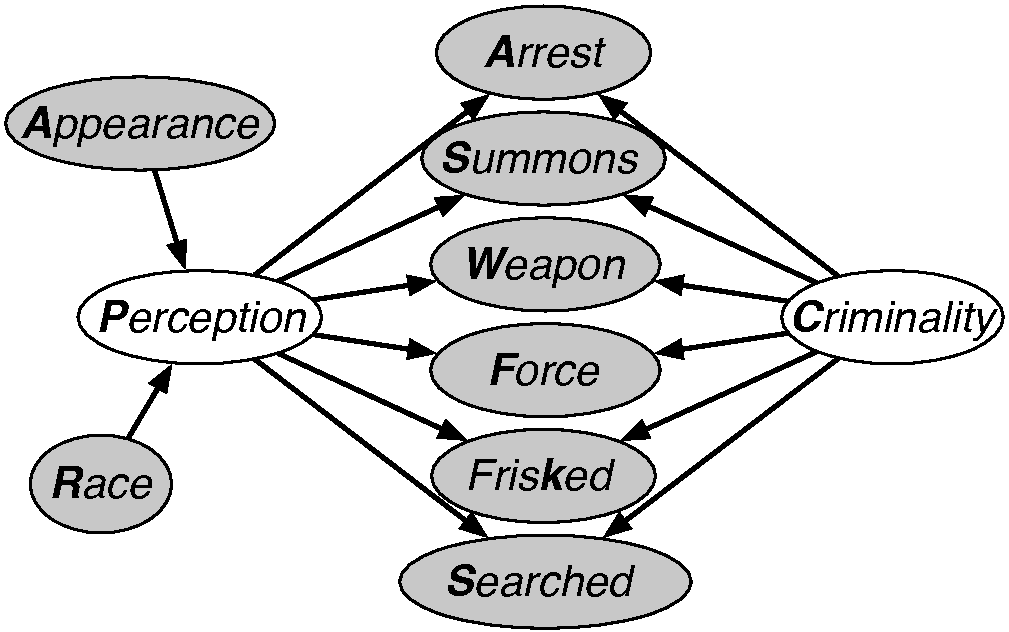
\includegraphics[width=3in]{stop_and_frisk_model3.pdf}}
\caption{A causal model for the stop and frisk dataset.\label{figure.stop_and_frisk}}
\end{center}
\end{figure}

\section*{S5 The Multifaceted Dynamics of Fairness}
\label{sec:dynamics}

One particularly interesting question was raised by one of the
reviewers: what is the effect of continuing discrimination after fair
decisions are made?  For instance, consider the case where banks
enforce a fair allocation of loans for business owners regardless of,
say, gender. This does not mean such businesses will thrive at a
balanced rate if customers continue to avoid female owned business at
a disproportionate rate for unfair reasons. Is there anything useful
that can be said about this issue from a causal perspective?

The work here proposed regards only what we can influence by changing
how machine learning-aided decision making takes place at specific
problems. It cannot change directly how society as a whole carry on
with their biases. Ironically, it may sound unfair to banks to enforce
the allocation of resources to businesses at a rate that does not
correspond to the probability of their respective success, even if the
owners of the corresponding businesses are not to be blamed by
that. One way of conciliating the different perspectives is by
modeling how a fair allocation of loans, even if it does not come
without a cost, can nevertheless increase the proportion of successful
female businesses compared to the current baseline. This change can by
itself have an indirect effect on the culture and behavior of a
society, leading to diminishing continuing discrimination by a
feedback mechanism, as in affirmative action. We believe that in the
long run isolated acts of fairness are benefitial even if we do not
have direct control on all sources of unfairness in any specific
problem.  Causal modeling can help on creating arguments about the
long run impact of individual contributions as e.g. a type of
macroeconomic assessment. There are many challenges, and we should not
pretend that precise answers can be obtained, but in theory we should
aim at educated quantitative assessments validating how a systemic
improvement in society can emerge from localized ways of addressing
fairness.

\section*{S6 Case Study: Criminality vs. Perceived Criminality}
\label{sec:true-vs.-perceived}

We test our approach on a problem of \emph{separating actual and
  perceived criminality in police stops}. For this problem, we
construct a causal model, and make explicit how unfairness may affect
observed and unobserved variables in the world. Given the model we
derive counterfactually fair predictors, and predict latent variables
such as a person's `criminality' (which may be useful for predicting
crime) as well as their `perceived criminality' (which may be due to
prejudices based on appearance). Finally we judge how well our
counterfactually fair `criminality' score satisfies demographic
parity.

\begin{figure}[!th]
\begin{center}
%\vspace{-1ex}
\centerline{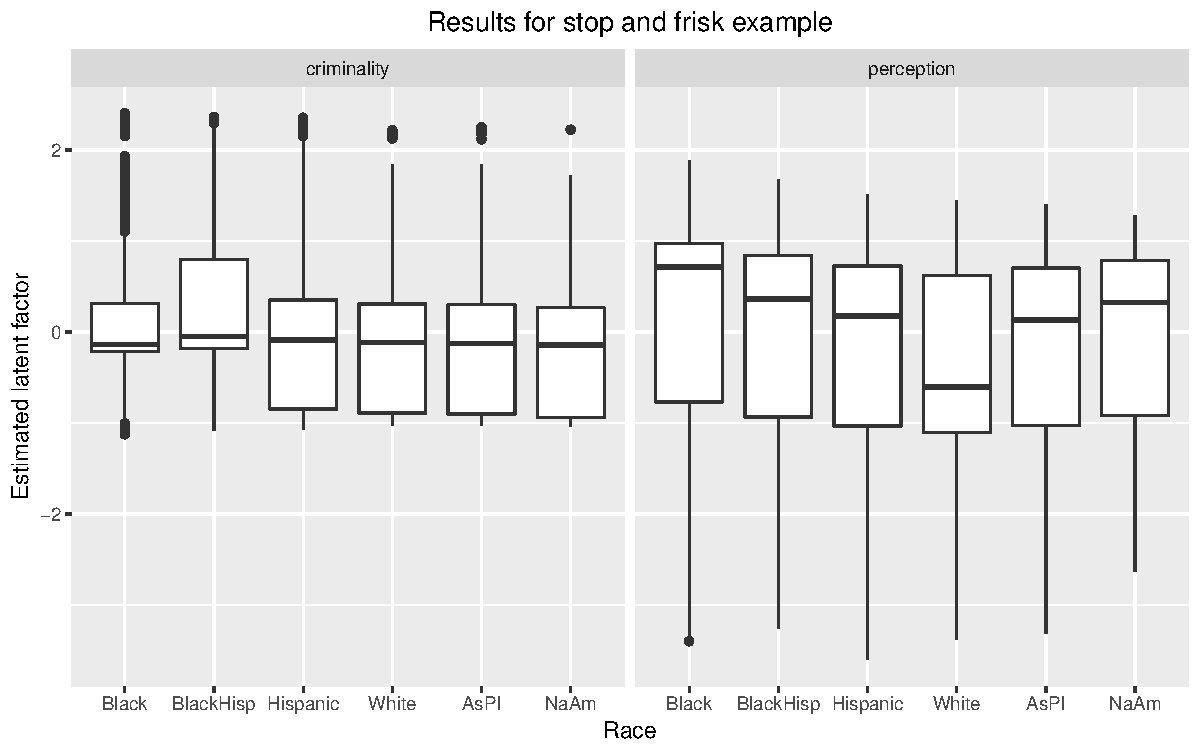
\includegraphics[width=4in]{stopandfrisk_output.pdf}}
\vspace{-2ex}
\caption{Distributions of estimated latent perception and criminality
  scores for the stop and frisk
  dataset.
\label{figure.stop_and_frisk_output}}
%\vspace{-2ex}
\end{center}
\end{figure}

Since 2002, the New York Police Department (NYPD) has recorded
information about every time a police officer has stopped someone. The
officer records information such as if the person was searched or
frisked, % if a weapon was found, their appearance, whether an arrest
was made or a summons issued, % if force was used, etc. We consider
the data collected on males stopped during 2014 which constitutes
38,609 records. % We limit our analysis to looking at just males
stopped as this accounts for more than $90\%$ of the data.  We fit a
model which decomposes these records into two latent factors, one
which depends on the race and appearance of the individual being
stopped, labeled \emph{Perceived Criminality}, and one which does not,
labeled \emph{Criminality}, and which could be used as a basis for
counterfactually fair decisions. We now describe a spatial analysis of
the estimated latent factors.

\paragraph{Model.}
We model this stop-and-frisk data using the graph in
Figure~\ref{figure.stop_and_frisk}. Specifically, we posit main causes
for the observations: \emph{Arrest} (if an individual was arrested),
\emph{Summons} (an individual was called to a court-summons),
\emph{Weapon} (an individual was found to be carrying a weapon),
\emph{Force} (some sort of force was used during the stop),
\emph{Frisked}, and \emph{Searched}. The first cause of these
observations is some measure of an individual's latent
\emph{Criminality}, which we do not observe. We believe there is an
additional cause, an individual's perceived criminality,
\emph{Perception}, also unobserved. This second factor is introduced
as we believe that these observations may be biased based on an
officer's perception of whether an individual is likely a criminal or
not. This perception is affected by an individual's \emph{Appearance}
and their \emph{Race}. In this sense \emph{Criminality} is
counterfactually fair, while \emph{Perception} models how race affects
each of the other observed variables.

\paragraph{Criminality and perception distributions.}
After fitting this model to the data we can look at the distribution
of \emph{Criminality} and \emph{Perception} across different races,
shown as box plots in Figure~\ref{figure.stop_and_frisk_output}. We see that
the median criminality for each race is nearly identical, while the
distributions are somewhat different, demonstrating that
\emph{Criminality} approaches demographic parity. The differences that
due exist may be due to unobserved confounding variables that are
affected by race or unmodeled noise in the data. On the right
\emph{Perception} varies considerably by race with white individuals
having the lowest perceived criminality while black and black Hispanic
individuals have the highest.

\begin{figure*}[!t]
\begin{center}
\centerline{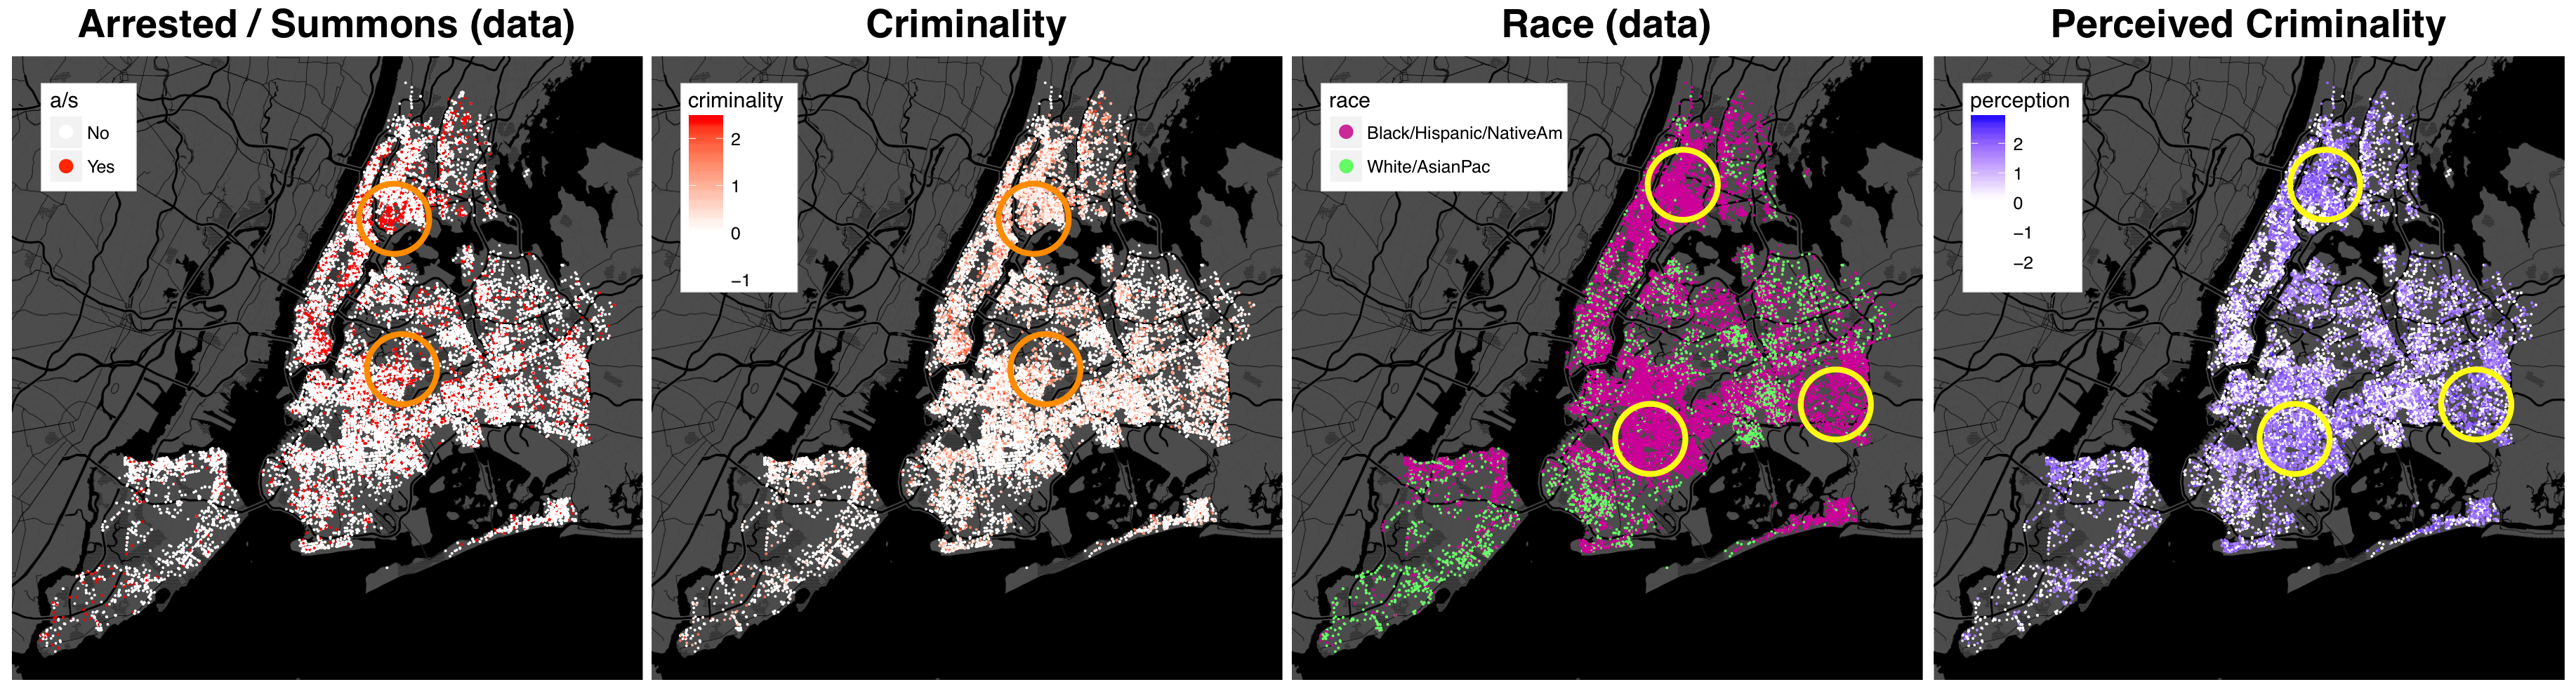
\includegraphics[width=\textwidth]{stop_and_frisk_graphs.png}}
\caption{Understanding criminality. The above maps show the
  decomposition of stop and search data in New York into factors based
  on perceived criminality (a race dependent variable) and latent
  criminality (a race neutral measure). \label{figure.criminality}}
\end{center}
\end{figure*}

\paragraph{Visualization on a map of New York City.}
Each of the stops can be mapped to longitude and latitude points for
where the stop
occurred\footnote{https://github.com/stablemarkets/StopAndFrisk}. Thus
we can visualize \emph{Criminality} and \emph{Perception} alongside
\emph{Race} and the combination of \emph{Arrest} and \emph{Summons},
shown in Figure~\ref{figure.criminality}.  Criminality seems to be a
continuous approximation of arrest and summons as both plots show red
in similar areas. However, the plots show that certain areas, while
having a lot of arrests have low criminality scores such as south
Bronx and west Queens (circled in orange). We can also compare the
perceived criminality with a plot of race, where we have divided the
races into Group A: black, black Hispanic, Hispanic, and Native
American (shown in purple); and Group B: white and Asian/Pacific
Islander (shown in green). Group A are all races that have positive
weights on the connection from \emph{Race} to \emph{Perception} in the
fitted model, while Group B all have negative weights. Thus being in
Group A leads one to have a higher perceived criminality than being in
Group B. This can be seen in the right-most plot of
Figure~\ref{figure.criminality}. Certain areas of town such as central
Brooklyn, central Bronx, and southern Queens have very high
criminality and almost all stops are by members of Group A (circled in
yellow).

%\subsection{Model criticism}
%%% Local Variables:
%%% mode: latex
%%% TeX-master: "ricardo_draft"
%%% End:
